
\chapter{Aplicaciones del análisis de Fourier}
\section{Desarrollo de Fourier}
\textbf{Idea del análisis de Fourier:} "toda" señal se puede descomponer en "tonos puros" (armónicos) de frecuencia fija (típicamente $\sin(\alpha n x)$ , $\cos(\alpha n x)$  $ n \in \ent$).

%Dibujo con caption ($\frac{1}{4} - \frac{2}{\pi^2} \sum_{n impares} \frac{1}{n^2} \cos(2\pi n x)$)

\begin{example}
Sea la función $f(t)=t$, $t\in[0,1)$ que se ha extendido periódicamente con período $T=1$.

\begin{center}
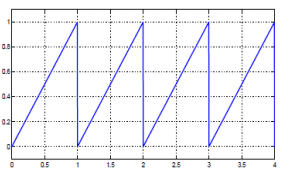
\includegraphics[width=\linewidth]{img/id_period.png}
\end{center}

Su desarrollo de fourier (que veremos más adelante cómo se calcula) queda de la forma:
\[SF(f(t))=\frac{1}{2}-\frac{1}{π}\sum_{n=1}^{\infty}\frac{1}{n}\sin(2πnt)\]

Cuántos más elementos del sumatorio tomemos más precisa será la proximación:

\begin{center}
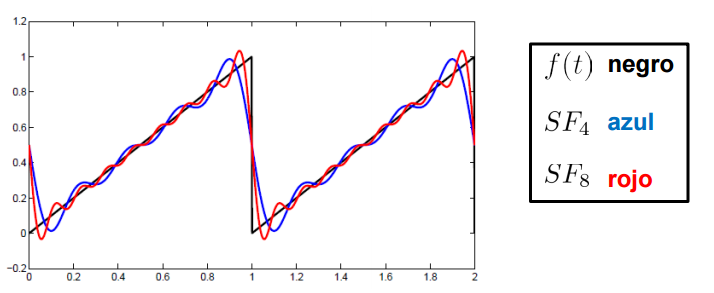
\includegraphics[width=\linewidth]{img/id_period_fourier.png}
\end{center}

	%Cogemos $x=0$:
	%$$0 = \frac{1}{4} - \frac{2}{\pi^2} \sum_{\text{n impares}} \frac{1}{n^2}$$
	%$$1 + \frac{1}{3^2} + \frac{1}{5^2} + \ldots = \frac{\pi^2}{8}$$
\end{example}

\subsection{Aplicaciones}
\begin{itemize}
	\item Muchas aplicaciones de ingeniería están basadas en estas ideas. (JPEG,(MP3) MPEG, telecomunicaciones)

	Hay tonos puros (frecuencias) que se eliminan o modifican porque no tienen mucha influencia o son ruido.

	Menos frecuencia $\rightarrow$ Menos información $\rightarrow$ Compresión (pérdidas)

	En ingeniería una aplicación muy común es utilizar esto como filtro, en el caso del MP3 se eliminan las frecuencias que no oimos.

	\item En matemáticas y física: Hay problemas difíciles para funciones generales y fáciles para "tonos puros" (senos y cosenos).

		\textbf{Interpretación de Copenhague}: Las partículas tienen funciones de ondas y en los experimentos solo se detectan los tonos puros que componen estas funciones con una probabilidad que depende de su amplitud.

	%Vamos a ver aplicaciones de esto:

	%\textbf{\textit{Pasar de analógico a digital}}

	%Vamos a hacer análisis de Fourier discreto con ondas digitalizadas.

%	\begin{example}
%		Vamos a estudiar la función $\sin\left(\frac{2\pi}{T}\cdot x\right)$
%
%		Dibujo
%
%		que es un caso particular de $\sin\left(\frac{2\pi}{T}\cdot k x\right)$ (oscila k veces en [0,T]).

%		Dibujo

%		Si digitalizamos la función, hacemos que x solo tenga valores discretos: $\sin\left(\frac{2\pi}{T}\cdot n\right)$

%		Dibujo

%		LLamamos $f(n)$ a la función discretizada, $n \in \ent$ ; Con N periódica $f(n + N) = f(n)$

%		Matemáticamente pensamos $f(n)$ como :
%		$$f : \ent/N\ent \rightarrow \mathbb{C} $$
%	\end{example}
	\obs En general consideramos que el recorrido de $f$ es $\mathbb{C}$ porque $e^{ix} = \cos x + i\sin x$ permite escribir senos y cosenos al mismo tiempo.

	$$\cos x = \frac{e^{ix} + e^{-ix}}{2}$$
	$$\sin x = \frac{e^{ix} - e^{-ix}}{2i}$$

\end{itemize}

\begin{theorem}[Análisis de Fourier en $\ent/N\ent$]

	Cualquier $f : \ent/N\ent \rightarrow \mathbb{C}$ se puede escribir como :
	$$f(n) = \frac{1}{N}\sum_{m\in \ent/N\ent}\widehat{f}(m)\cdot e\left(\frac{nm}{N}\right)$$
	donde $e(x) = e^{2\pi ix}$

	$\widehat{f}(n)$ es la \textbf{transformada de Fourier discreta}
	$$\widehat{f}(n) = \sum_{m\in \ent/N\ent}\widehat{f}(m)\cdot e\left(\frac{-nm}{N}\right)$$

\end{theorem}
\obs Hay un algoritmo (FFT) para calcular los $\widehat{f}(m)$

\begin{proof}
	Definimos la función $\delta : \ent/N\ent \rightarrow \mathbb{C}$ como :
	$$\delta (n) = \begin{cases}
	1 \text{ si } n=0\\
	0 \text{ si } n\neq 0 \\
	\end{cases}$$
	Y decimos que también se puede escribir como:
	$$\delta (n) = \frac{1}{N} \sum_{m = 0}^{N-1} e\left(-\frac{nm}{N}\right)$$
	Donde
	\[e\left(\frac{nm}{N}\right) = e^{\frac{2\pi inm}{N}}\]

	Es claro que $\delta(0) = 1$, pero aún tenemos que ver que $n\neq 0 \implies \delta (n) = 0$

	Podemos ver δ como el producto de $\frac{1}{N}$ por la suma de los términos de una progresión geométrica tal que:
	\[\begin{cases}
	a_1 = e(n0/N)=e(0)=1\\
	a_{n+1} = e(-nN/N)=e(n)\\
	\text{razón } = e^{-\frac{n}{N}}
	\end{cases}\]

	Basándonos en la fórmula conocida para la suma de los términos de una progresión geométrica tenemos:
	$$\delta (n) =\frac{e^{n} - e(0)}{e^{n/N} - 1} = 0$$

	Otra forma de pensarlo es como vectores. $\delta(n)$ se puede ver como la suma de todas las raíces de la unidad. Sumando todas las fuerzas vemos que se anulan.

	%(dibujo explicativo para N=4)

	Una vez que tenemos esto, vemos que la $f(n)$ de la proposición se puede escribir como:
	$$f(n) = \sum_{k\in \ent/N\ent} f(k) \cdot \delta(n-k)$$
	Sustituyendo:
	$$f(n) = \frac{1}{N} \sum_{k\in \ent/N\ent} f(k)  \sum_{m \in \ent/N\ent} e\left(\frac{nm}{N}\right) \cdot e\left(- \frac{km}{N}\right)$$

	Y como por definición:
	$$\widehat{f}(m) = \sum_{k\in \ent/N\ent} f(k) \cdot e\left(- \frac{km}{N}\right)$$

	Pues ya está probada la proposición.
\end{proof}
\begin{example}
	Un ejemplo de esto con N=3

	DIBUJO

	Vemos que la función se va repitiendo po lo que cojo solo el tramo de 0 a 2 para estudiarla.
	$$f(n) = \begin{cases}
	7 si n= 0\\
	2 si n = 1 , 2
	\end{cases}$$

	Entonces aplicando la proposición nos queda:
	$$\widehat{f}(0) = f(0)\cdot e(0) + f(1)\cdot e(0) + f(2) \cdot e(0) =  11$$
	$$\widehat{f}(1) = f(0)\cdot e(0) + f(1)\cdot e\left(-\frac{1}{3}\right) + f(2)\cdot e\left(-\frac{2}{3}\right) = 7 + 2\cdot\left(-\frac{1}{2} -i\frac{\sqrt{3}}{2}\right) + 2\cdot \left(-\frac{1}{2} + \frac{i\sqrt{3}}{2}\right) = 5$$
	$$\widehat{f}(2) = f(0)\cdot e(0) + f(1)\cdot e\left(- \frac{2}{3}\right) + f(2) \cdot e\left(-\frac{4}{3}\right) = 7 + 2\cdot\left(-\frac{1}{2} -i\frac{\sqrt{3}}{2}\right) + 2\cdot \left(-\frac{1}{2} + \frac{i\sqrt{3}}{2}\right) = 5$$
	Como
	$$f(n) = \frac{1}{N} \sum_{m\in \ent/ N\ent} \widehat{f}(m) \cdot e\left(\frac{nm}{N}\right)$$
	Sustituyendo con los resultados de antes nos queda que:
	$$f(n) = \frac{11}{3}\cdot e\left(0 \frac{n}{3}\right) + \frac{5}{3}\cdot e\left(1 \frac{n}{3}\right) + \frac{5}{3} \cdot e\left(2 \frac{n}{3}\right)$$

	Y efectivamante, si comparamos resultados nos queda :
	$$n = 0 \rightarrow 7 = \frac{11}{3} + \frac{5}{3} + \frac{5}{3}$$
	$$n = 1 \rightarrow 2 = \frac{11}{3} + \frac{5}{3} \cdot \left(- \frac{1}{2} + \frac{i \sqrt{3}}{2}\right) + \frac{5}{3} \cdot \left(- \frac{1}{2} -\frac{i \sqrt{3}}{2}\right)$$
\end{example}

Esta proposición se puede utilizar para \textbf{transformar funciones discretas(con N grande) a funciones continuas}.

DIBUJOS DE LA F DISCRETA Y CONTINUA

Tenemos f(n) discreta, llamamos $F\left(\frac{n}{N}\right) = f(n)$ a la función continua que queremos construir.


Haciendo el desarrollo de Fourier de f nos queda que:
$$f(n) = \sum \frac{\widehat{f}(m)}{N} \cdot e\left(\frac{nm}{N}\right)$$

Llamamos $x = \frac{n}{N}$ y $a_m= \frac{\widehat{f}(m)}{N}$ y nos queda que :
$$F(x) = \sum_{n\in \ent } a_m \cdot e(mx)$$

Para calcular $F(x)$ necesitamos calcular primero el $a_m$. Para ello hacemos el límite de $\frac{\widehat{f}(m)}{N}$

Entonces tenemos que:
$$\frac{\widehat{f}(m)}{N} = \frac{1}{N} \sum_{k \in \ent/N\ent} f(k) \cdot e\left(-m \frac{k}{N}\right) \rightarrow \begin{cases}
	m \text{ fijo}\\
	N \text{ muy grande}\\
	f(k) = F\left(\frac{k}{N}\right)\\
\end{cases}$$

Como $ k = 0 , \ldots , N-1 \implies 0\leq \frac{k}{N} < 1$ podemos tomar el sumatorio como suma de Riemann.

$$\frac{\widehat{f}(m)}{N} = \int_{0}^{1} F(x) \cdot e(-mx) dx$$

Entonces
$$F(x) = \sum_{m= -\infty}^{\infty} \widehat{F}(n) \cdot e(nx)$$
Siendo $\widehat{F}(n) = \int_{0}^{1} F(x) \cdot e(-nx) dx$

Y si F es buena ( p.ej $C^2$) entonces todo funciona bien.
Si no es buena hay casos donde no fuciona.



%%% CLASES POR  REVISAR



$ f: \mathbb{R} \rightarrow \mathbb{C} $ 1-periódica

$f(x) = \sum\limits_{n=-\infty}^{\infty} \hat{f}(n) e(nx) \;\;\;\;\;\; \hat{f}(n) = \int\limits_{0}^{L} f(x) e (-nx) dx \;\;\;\; e(x) = e^{2 \pi i x}$

$f(x) \equiv $ Desarrollo de Fourier de f \;\;\;\; $\hat{f}(n) =$ coeficientes de Fourier de f.

La igualdad $f(x) = \sum^{\infty}_{n=-\infty}$ es cierta para $f$ periódica $\in C^{2}$ y la convergencia es uniforme (Tma. de Carlesson-Hunt $\Rightarrow$ la igualdad es cierta en casi todo punto con tal de que $f \in L^{P} [0,1] p > 1$)

¿Se puede analizar en senos y cosenos una función no periódica? Sí, pero hay que tomar los de frecuencias no enteras.

$g \equiv $ función 1-periódica $ \Rightarrow f(x) = g(\frac{x}{T})$ es T-periódica.

$$ g(x) = \sum^{\infty}_{n=-\infty} \hat{g}(n) e(nx) \;\;\; \hat{g}(n) = \int\limits^{1}_{0} = \int\limits^{1/2}_{-1/2} g(x) e(-nx) dx $$

$x |\rightarrow \frac{x}{T} $

$$f(x) = \sum_{n = -\infty}^{\infty} \hat{g}(n) e(\frac{n}{T}x) \;\;\; \hat{g}(n) = \frac{1}{T} \int\limits^{T/2}_{-T/2} f(y) e(-\frac{n}{T}y) dy$$

$$f(x) = \frac{1}{T} \sum_{n = -\infty}^{\infty} \left(  \int\limits^{T/2}_{-T/2} f(y) e(-\frac{n}{T}y) dy \right) e (\frac{n}{T}x)$$

$T \rightarrow \infty$ Escribiendo $\frac{n}{T} = \psi$

$$ f(x) =^{?} \int\limits^{\infty}_{-\infty} \text{ otra integral } e(\psi x) d\psi $$

Esto sugiere que para $f: \mathbb{R} \rightarrow \mathbb{C}$

$$f(x) = \int\limits^{\infty}_{-\infty} \hat{f}(\psi) e (x \psi) d \psi \text{ donde } \hat{f}(\psi) = \int\limits^{\infty}_{-\infty} f(y) e(-\psi y)dy$$

$\hat{f}$ se conoce como la transformada de Fourier (y se inventó antes que la discreta). Y $f(x)$ es la Fórmula de inversión.

La igualdad $f(x) = \int\limits^{\infty}_{-\infty} $... es cierta para $f$ que decaiga rápido con cierta regularidad.


RESUMEN:

\begin{itemize}

\item Si tenemos una función $f$ : $\mathbb{Z}_{n} = \mathbb{Z} / n \mathbb{Z} \rightarrow \mathbb{C}$

$$ f(n) = \frac{1}{n} \sum_{m \in \mathbb{Z}_{n}} \hat{f}(m) e \left( \frac{mn}{N} \right) $$

$$ \hat{f}(n) = \sum_{m \in \mathbb{Z}_{n}} f(m) e \left( \frac{-mn}{N} \right)$$

\item Para $f: \mathbb{T} \rightarrow \mathbb{C} \;\;\;\; \mathbb{T} = \mathbb{R}/\mathbb{Z}$.  $x$, $x+n$ se identifican $f$: $\mathbb(T) \rightarrow \mathbb{C}$ = functiones 1-periódicas.

$$ f(x) = \sum{\infty}_{n = -\infty} \hat{f} (n) e (nx) $$

$$ \hat{f} (n) = \int\limits_{0}^{1} f(x) e (-nx) dx $$

\item Para f: $\mathbb{R} \rightarrow \mathbb{C}$

$$ f(x) = \int\limits^{\infty}_{-\infty} \hat{f}(\psi) e(x \psi) d\psi $$

$$ \hat{f}(\psi) = \int^{\infty}_{-\infty} f(x) e(-\psi x)dx$$

\end{itemize}

\begin{obs}

	Para la segunda y la tercera necesitamos cierta regularidad.

\end{obs}


\begin{example}

	Hallar el desarrollo de Fourier de la función 1-periódica que en $[-1/2, 1/2]$ vale $e^{2\pi x} + e^{-2\pi x } = 2 \cosh (2 \pi x)$

	(DIBUJO CATENARIA PERIÓDICA)


	$$\hat{f}(n) = \int ^{1/2}_{-1/2} \left( e^{2 \pi x} + e ^{-2 \pi x} \right) e ^{-2 \pi i n x = e (-nx)} = \frac{1}{2 \pi} (e^{\pi} - e^{-\pi}) (-1)^{n} \left( \frac{1}{1-in} + \frac{1}{1 + in} \right) $$

	$$ = \frac{e^{\pi} - e^{-\pi}}{\pi} (-1)^{n} \frac{1}{1 + n^2}$$

	$$ f(x) = e ^{2 \pi x} + e^{-2 \pi x} = \frac{e^{pi} - e^{-\pi}}{\pi} \sum_{n = -\infty}^{\infty} \frac{(-1)^n}{1 + n^2} e(nx) $$

\end{example}












\begin{example}{Otro ejemplo}

Expresar $e^{-|x|}$ como una integral usando la fórmula de inversión.


Recordemos la fórmula de inversión:

$$ f(x) = \int\limits^{\infty}_{-\infty} \hat{f}(\psi) e(x\psi) d\psi \rightarrow \hat{f}(\psi) = \int\limits^{\infty}_{-\infty} f(x) e(-\psi x) dx$$

Entonces:

$$f(x) = e^{-|x|} \;\;\;\;\;\; \hat{f}(\psi) = \int_{-\infty}^{\infty} e^{-|x|} e ^{-2 \pi i \psi x} dx = $$

$$ \int_{0}^{\infty} e ^{-(1 + 2 \pi i \psi) x} + \int_{-\infty}^{0} e ^{(1 - 2 \pi i \psi) x} = \frac{1}{1 + 2\pi i \psi} + \frac{1}{1-2 \pi i \psi} = \frac{2}{1 + 4 \pi^2 \psi^2}$$


$$e^{-|x|} = \int\limits_{-\infty}^{\infty} \frac{2 e (x \psi)}{1 + 4 \pi^2 \psi^2} d \psi = \int\limits^{\infty}_{-\infty} \frac{2 cos(2 \pi x \psi)}{1 + 4 \pi^2 \psi^2} d\psi $$

\end{example}

\section{Proyecciones, convoluciones y filtros}

$V =$ espacio vectorial euclideo (complejo)

$\{\vu_1, ..., \vu_n\}$ base ortonormal.

$\vx \in V \Rightarrow \vx = \lambda_1 \vu_1 + ... \lambda_n \vu_n$

Como la base es ortonormal es muy facil de calcular los $\lambda_i$: $\lambda_i = <\vu_i, \vx>$

Además tenemos que la proyección dobre el subespacio $S$ que genera $\{\vu_1,...,\vu_k\}$ es:

$ P_{r_s}(\vx) = <\vu_1, \vx>\vu_1 + ... + <\vu_k, \vx>\vu_k $ (porque es ortonormal)

$ P_{r_s}(\vx) \equiv $ proyección de $\vx$ sobre S.

$ V = \{f: \mathbb{Z}_n = \mathbb{Z}/n\mathbb{Z} \rightarrow \mathbb{C} \} $

$<f, g> = \frac{1}{N} \sum_{n \in \mathbb{Z}_n} \conj{f(n)} g(n)$


\begin{prop}
	$f_m(n) = e\left(\frac{nm}{N}) \right) $ Las funciones $\{ f_0, f_1, ..., f_{n-1}\}$ son una base ortonormal

\end{prop}

\begin{proof}

	$<f_m, f_{m'}> = \frac{1}{N} \sum^{n-1}_{n = 0} e \left(-\frac{nm}{N} \right) e \left(\frac{nm'}{N} \right) = \frac{1}{N} \sum^{n-1}_{n = 0} e \left( \frac{n (m' - m)}{N} \right) =$

	$$ = \delta (m' - m) = \begin{cases}
		0 \mbox{si} m' \neq m \\
		1 \mbox{si} m' = m
	\end{cases}
	$$

	Cualquier $f$ cumple $f = \sum^{N - 1}_{m = 0} \lambda_m f_m = <f_m, f> \Leftrightarrow_{1 ref} f(n) = \frac{1}{N} \sum_{m \in \mathbb{Z}_n} \hat{f}(m) e(\frac{nm}{N}) $

\end{proof}

\begin{prop}

	$\mathbb{T}$: solo es una forma de identificar $x$ con $x+n$.

	$V = \{ f: \mathbb{T} \rightarrow K, f \in L^2 [0,1]\} \;\;\;\;\; <f,g> = \int\limits^{1}_0 \conj{f(x)} g(x) dx $

	$f_n(x) = e(nx)$ son ortonormales.

\end{prop}

\begin{proof}

	$$< f_n, f_{n'}> = \int\limits^1_0 e(-nx) e(n'x) dx = \int^1_0 ((n' -n)x) dx =
	\begin{cases}
		1 \mbox{si} n = n'
		0 \mbox{si} n\neq n'
	\end{cases}$$

	En todo esto nos falta decir que los $f_n$ son una base:

	Si los $f_n$ fueran una base (también llamado sistema ortonormal completo) entonces:

	$$f = \sum_{n \in \mathbb{Z}} \lambda_n f_n \;\;\;\;\;\; \lambda_n <f_n, f> = \int\limits^{1}_0 e(-nx) f(x) dx = \hat{f(n)}$$

	Y esto equivale a 2 (falta referencia)

\end{proof}

\begin{prop}

	El caso 3 (ref) es un poco diferente pero análogo con $<f,g> = \int^{\infty}_{-\infty} \conj{f(x)} g(x) dx$

\end{prop}

\begin{corol}
	De esta forma podemos aplicar ideas de álgebra lineal

	$\vx = <\vu_1, \vx>\vu_1 + ... + <\vu_n, \vx>\vu_n$

	$\norm{\vx}^2 = \abs{<\vu_1, \vx>}^2 + ... + \abs{<\vu_n, \vx>}^2$

	En el caso 2 (ref)

	$\norm{f}^2 = \int^1_0 \abs{f}^2 = \sum_{n \in \mathbb{Z}} \abs{\hat{f}(n)}^2 \rightarrow$ Identidad de par se val


\end{corol}







Proyeccion usasa en audio: en vez de $-\infty$ a $\infty$, 20 a 20000

Más general es atenuar o amplificar los coeficientes de Fourier dependiendo de sus frecuencias

Entonces el proceso de compresión se realiza usando alguna regla que efectue:

$f(x) = \sum\limits^{\infty}_{n = -\infty} a_n e(nx) \rightarrow \sum\limits^{\infty}_{n = - \infty} W(n) a_n e(nx)$

La mayor parte de las aplicaciones del análisis de Fourier se basan en procesos de este tipo.

Se está asignando un peso a cada una de las frecuencias. Como con los filtros de paso alto, bajo, banda...

¿Que le ocurre a la función tras transformarla de esta manera? ¿Hay alguna relación simple entre f y la señal transformada? (Sin el desarrollo de Fourier)

Sí, a través de convoluciones

\begin{defn}{Convolución}
	Se llama convolución de $f$ y $g$, y se escribe $f*g$ a:
	\begin{itemize}
		\item $fg :\mathbb{Z}_{N} \rightarrow \mathbb{C} \;\;\; (f * g)(n) = \sum\limits_{m \in \mathbb{Z}_{N}} f(n-m)g(m)$
		\item $fg :\mathbb{T} \rightarrow \mathbb{C} \;\;\; (f * g)(x) = \int\limits^{1}_{0} f(x-t)g(t)dt$
		\item $fg :\mathbb{R} \rightarrow \mathbb{C} \;\;\; (f * g)(x) = \int\limits^{\infty}_{-\infty} f(x-t)g(t)dt$
	\end{itemize}

\end{defn}

\begin{obs}

$f =$ señal $f = $ (DIBUJITO)

Convolver es como multiplicar por trasladados y promediar usando $g$.


(MAS DIBUJITOS (puntos sueltos)) -> resultado = promedio de "anchura" 3 de la señal.

%\begin{figure}[htbp]
%	\centering
%	\subfigure[Función f discontinua]{\inputtikz[width=80mm]{fourier/funcionFConvolucion}}
%	\subfigure[Función g continua]{\inputtikz[width=80mm]{fourier/funcionGConvolucion}}
%	\caption{Regularizar funciones}
%\end{figure}

(IMAGEN DE UNA F DISCONTINUA Y UNA G CONTINUA QUE REGULARIZA)



ejemplo: filtro gaussiano. Las cosas pierden cambios bruscos. se convoluciona con una campana de gauss.

También se pueden detectar bordes.

\end{obs}


\begin{prop}
	Se cumple $\hat{f*g} = \hat{f} \hat{g}$.

	Es decir, multiplicar los coeficientes de Fourier (o tranaformadas de Fourier) por $\hat{g}$ es lo mismo que convolver la señal con $g$.

\end{prop}

\begin{proof}
	\textit{Usaremos el caso 3, las demostraciones en los otros casos son similares a ésta}

$$ \hat{f*g}(\psi) = \int\limits^{\infty}_{-\infty} (f*g)(x) e(-x\psi)dx $$
$$ = \int\limits^{\infty}_{-\infty} f(x - t) e (-x \psi) dx dt \;\;\;\; x = y + t$$
$$ = \int\limits^{\infty}_{-\infty} g(t) \int\limits^{\infty}_{-\infty} f(y) e (-y \psi) e(-t\psi)dy dt$$

$$ \int\limits^{\infty}_{-\infty} g(t) e(-t\psi) dt = \hat{g}(\psi) \;\;\;\;\;\;\; \int\limits^{\infty}_{-\infty} f(y) e (-y \psi) dy = \hat{f}(\psi) $$

$$\hat{f*g} (\psi) = \hat{f}(\psi) \hat{g}\psi $$

\end{proof}



\subsection{Simtrías, regularidad y convergencia}


(UNOS TRIANGULOS DIVIDIDOS A LA MITAD VERTICALMENTE)

$$ = \frac{1}{4} - \frac{2}{\pi^2} \sum_{\text{n impar}} \frac{cos(2 \pi n x)}{n^2}$$

los coeficientes decaen como $n^{-2}$

$$ \sum_{n < N} \rightarrow \text{ error } \leq \sum_{n \geq N} \frac{1}{n^2}  ≈ N^{-1} $$



(DIBUJO SIERRA)

$$ = \frac{1}{2} - \frac{1}{\pi} \sum^{\infty}_{n = 1} \frac{sen(2 \pi n x)}{n}$$

$ \sum_{n > N} \rightarrow \sum_{n > N} \frac{1}{n}$ ni siquiera converge (1)

La regularidad influye en la rapidez de convergencia de la serie de Fourier.




¿Porqué ocurre que la función que da el diente de sierra es? : $\frac{1}{2} - \frac{1}{\pi} \sum_{n=1}^{\infty} \frac{\sin(2\pi nx)}{n}$

Esta suma se puede probar que converge(pero la demostración no es fácil en absoluto) pero, excepto para $x = \frac{k}{2}$, se puede probar que la convergencia no es absoluta.

\subsection{Convergencia lenta:} es malo para las aplicaciones porque no podemos despreciar muchos coeficientes de Fourier.

	Si tengo una función $f: \ent_N \rightarrow \mathbb{C}$
	$$f(n) = \frac{1}{N}\sum_{m \in \ent_N}\widehat{f}(m)e(\frac{mn}{N})$$

	Para N grande y coeficientes parecidos $\implies$ es difícil decidir cuáles omitir.

	Vamos a suponer que tenemos una función 1-periódica $f : \Pi \rightarrow \mathbb{C}$ tal que $f \in C^{\infty}(\mathbb{R})$.

	Para $n \neq 0$

	$$\widehat{f}(n) = \int_{0}^{1} f(x) e(-nx) dx$$

	Llamamos $\begin{cases}
	u = f(x)\\
	dv = e(-nx) dx
	\end{cases}$

	Entonces:
	$$\widehat{f}(n) = f(x) \frac{e(-nx)}{-2\pi in}|_{0}^1 + \frac{1}{2\pi i n} \int_{0}^1 f'(x) e(-nx) dx$$

	Como $f(x) \frac{e(-nx)}{-2\pi in}|_{0}^1 $ es 0,como f es periódica, si seguimos iterando hasta k veces:

	$$\widehat{f}(n)  \frac{1}{(2\pi i n)^k} \int_{0}^1 f^{(k)}(x) e(-nx) dx$$

	y como $|f^{(k)}| \leq cte$ en [0,1] $\implies |\widehat{f}(n)| \leq \frac{cte}{|n|^k}$

	Con menos regularidad: $f^{(k)}$ existe excepto en un número finito de puntos (de [0,1]) y está acotada, daría el mismo resultado.

	Vamos a ver esto para $k=2$:

	$$k=2 \implies |\widehat{f}(n)| \leq cte \implies \sum_{n= -\infty}^{e(nx)}$$
	Converge absolutamente.


\begin{center}
	\centering
	\inputtikz{fourier/audioRepeticionNoContinua}
\end{center}

	La extensión 1-periódica de una función, típicamente no es nisiquiera continua. $\implies$ típicamente no se puede tomar $k=2$ $\implies$ malo para las aplicaciones.

	En estos casos se usa un truco, en lugar de la extensión periódica primero se refleja la función(la señal) por el eje Y.

	Y después se extiende de forma 2-periódica

	Como el reflejo y la señal original coinciden en el final de una y el principio de la otra esta extensión si sería continua


	\begin{center}
		\centering
		\inputtikz{fourier/audio_simetria_simple}
	\end{center}


	Entonces vamos a ver las ecuaciones de Fourier para las funciones 2-periódicas.

	$$f(x) = \sum_{n=-\infty}^{\infty} \widehat{f}(n)e(n\frac{x}{2})$$

	Siendo
	$$\widehat{f}(n) = \frac{1}{2} \int_{0}^{2} f(x) e(-nx)$$

	Estos números son reales si f es real.

	$$\widehat{f}(n) = \frac{1}{2} \int_{-1}^{1} f(x) e(-n\frac{x}{2}) dx = \frac{1}{2} \int_{-1}^{1} f(x)\cos(2\pi n \frac{x}{2})dx \in \mathbb{R}$$

	Eto es porque $e(-n\frac{x}{2}) = \cos(2\pi n \frac{x}{2}) + i \sin(2\pi n \frac{x}{2})$ y además f es par y $\sin$ es impar.

	¿Cómo adaptar esto al caso discreto $f: \ent_N \rightarrow \mathbb{C}$?

	\begin{center}
		\centering
		\inputtikz{fourier/extension_2_periodica}
	\end{center}

	Haciendo las cuentas se btiene un análisis de Fourirer discreto en el que podemos usar $e((m + \frac{1}{2}) \frac{n}{2N})$ en vez de $e(\frac{mn}{N})$ y tomando partes reales se puede escribir todo en términos $\cos(\frac{\pi n}{N}(m+ \frac{1}{2}))$

	\begin{prop}
		Para $f : \{0,1,2....,N-1\} \rightarrow \mathbb{R}$ se cumple
		$$f(m) = \frac{\widehat{f}^c(0)}{N} + \frac{2}{N} \sum_{n=1}^{N-1} \widehat{f}^c(n) \cos(\frac{n\pi}{N}(m + \frac{1}{2}))$$
		donde
		$$\widehat{f}^c(n)= \sum_{m= 0}^{N-1} f(m) \cos(\frac{n\pi}{N}(m+ \frac{1}{2}))$$
	\end{prop}
	\begin{obs} Y esto es lo que más se utiliza en tratamiento de señales de sonido, imagen....
	\end{obs}

	\begin{proof}
		Lo único que hay que hacer es sustituir la definición de $\hat{f}^c (n)$ y comprobar que se tiene una identidad.

		Vamos a abreviar:

		$$f(n) = \sum\limits^{N-1}_{m=0} f(m) \delta(n - m) \;\;\;\;\; \delta(n) = \begin{cases}
			0 & \mbox{si } n \neq 0 \\
			1 & \mbox{si } n = 0
		\end{cases}$$

		$f = $combinación lineal de $\delta{-m} \Rightarrow $ basta probar la fórmula para las funciones $f(n) = \delta(n- m_0)$.

		Si escribimos la propiedad para $f(n) = \delta(n - m_0)$ y usamos $2 \cos{(\alpha)} \cos{(\beta)} = \cos{(\alpha + \beta)} + \cos{(\alpha - \beta)}$, lo que hay que probar es:

		$$ \delta(m - m_0) \qeq \frac{1}{N} + \frac{1}{N} \sum\limits^{N-1}{n = 1} \left[ \cos{\frac{\pi n}{N} (m_0 + m + 1)} + \cos{\frac{\pi n}{N} (m - m_0)}   \right] $$

		$$ \delta(m - m_0) \qeq \frac{1}{N} + \frac{1}{N} \sum\limits^{N-1}{n = 1} \left[ \text{Re} \left( e \left( \frac{n}{2N} (m_0 + m + 1) \right) \right) + \text{Re} \left( e \left( \frac{\pi n}{2N} (m - m_0) \right) \right)   \right] $$

		Duplicaríamos la $n$ si añadimos los negativos o los $2N-1, 2N-2, 2N-3,...$.

		$$ = \frac{1}{2N} \text{Re} \sum\limits^{2N-1}_{n=0} \left( e \left( \frac{n}{2N} (m_0 + m + 1) \right) + e \left( \frac{\pi n}{2N} (m - m_0) \right) \right) $$

		$$ \sum\limits^{M - L}_{k = 0} e \left( \frac{k}{M} l \right) = \begin{cases}
			0 & \mbox{si } l \not\equiv 0 \; (M) \\
			M & \mbox{si } l' \equiv 0 \; (M)
		\end{cases}$$

		$\Rightarrow$ la expresión de arriba es $\delta(m - m_0).$

		(prueba supuestamente sencilla teniendo en cuenta que $m-m_0$ varía entre 0 y $N-1$)

	\end{proof}


\section{Aplicaciones}

	\subsection{Formato JPEG}

		\begin{center}
			\inputtikz{fourier/matriz_imagen}
		\end{center}

		Cada píxel son 3 números (bytes) (RGB) (si tiene transparencia 1 más correspondiente al canal alfa)

		R,G,B $\in$ [0,255] (enteros)

		Como hay combinaciones de R y G que se parecen demasiado para el ojo humano, en la realidad casi siempre se pasa de RGB a Y$\text{C}_{\text{B}}$ $\text{C}_{\text{R}}$ con un ``cambio de base'' = con una transformación lineal.

		\begin{itemize}
			\item Y = luminancia $\rightarrow$ el ojo es muy sensible a ella
			\item $\text{C}_{\text{B}}$ Crominancia $\rightarrow$ el ojo es poco sensible a ella.
			\item $\text{C}_{\text{R}}$ Crominancia $\rightarrow$ el ojo es poco sensible a ella.
		\end{itemize}


		En lo que respecta a $\text{C}_{\text{B}}$ y $\text{C}_{\text{R}}$ de omite píxeles (como considerar una foto escalada).

		Imágenes en tonos de gris $\rightarrow$ cada píxel tiene R=G=B y son igules a Y.Nos restringimos a este caso. El general es igual repetido 3 veces.

		\begin{center}
			\inputtikz{fourier/imagen_en_bloques}
		\end{center}

		La imagen $N \times M$ se divide en bloques $8 \times 8$. Cada uno de ellos se puede interpretar como una función:

		$f:\{0,1,...7\} \times \{0,1,...7\} \rightarrow \mathbb{R}$ que asigna al píxel $P_{ij}$ del bloque, su color (R,Y,G,B $\in [0,255]$) (solo un número para nuestro caso de tonos de gris).


		\textbf{Idea} Descomponer $f$ por Fourier y suprimir las frecuencias altas excepto si tienen coeficientes (amplitudes) grandes.









